%%%%%%%%%%%%%%%%%%%%%%%%%%%%%%%%%%%%%%%%%%%%%%%%
%
% start writing
%
%%%%%%%%%%%%%%%%%%%%%%%%%%%%%%%%%%%%%%%%%%%%%%%%


\chapter{Introduction}
\label{chap:Introduction}
\section{Background}
Since all systems are prone to failure, an engineer's responsibilities involve ensuring that crucial systems never fail and therefore that proper testing and continual maintenance is performed. In the case of satellites, the problem proves even more severe, since most failures are unrecoverable. Satellite systems must therefore be tested thoroughly and be robust to any anomaly. According to \cite{tafazoli2009study}, the attitude and orbit control system (AOCS) contributes to the largest percentage of satellite failures as shown in Figure~\ref{fig:OnOrbitFailureSubsystem}. A study conducted by \cite{Jacklin2019} on small satellite mission failures provides a deeper insight into the attitude control's role in satellite failures, since most missions are highly dependent on the attitude control for complete mission success. This is due to many mission specifications that rely on accurate control of the satellite to ensure that payloads, such as cameras, are able to operate as required.

%\begin{figure*}[!htb]
%	\centering
%	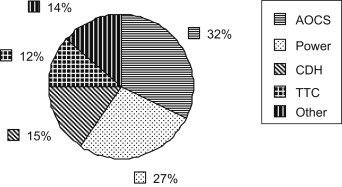
\includegraphics[width = 7cm]{Figures/OnOrbitFailureDistribution.jpg}
%	\caption{On-orbit failure per subsystem \cite{tafazoli2009study}}
%	\label{fig:OnOrbitFailureSubsystem}
%\end{figure*}

\begin{figure*}[!htb]
	\centering
	\begin{tikzpicture}
	\pie{32/AOCS,
		27/Power,
		15/CDH,
		12/TTC,
		14/Other}
	\end{tikzpicture}
	\caption{On-orbit failure per subsystem \cite{tafazoli2009study}}
	\label{fig:OnOrbitFailureSubsystem}
\end{figure*}

The database provided by \cite{swartwout2015cubesat} demonstrates the increase in the number of satellites launched every year. The drastic increase of launched satellites over the past few years further emphasizes this need of ensuring that satellites are robust to failures. Using traditional methods of tracking satellites with ground stations and manually checking for possible failures are therefore not feasible, especially in the case of satellite constellations. Consequently, most aspects of the satellite should operate autonomously, especially in the case of attitude control. The focus of this thesis is on a specific aspect of the attitude control which is sensitive to anomalies, namely the attitude determination. 

The extended Kalman filter (EKF) is implemented for attitude estimation of the satellite. The objective of this thesis is therefore to develop methods that can be used to avoid unstable and inaccurate estimations from the EKF caused by sensor anomalies.

\section{Problem Description}
For many satellite missions, attitude determination and control system (ADCS) is of high importance. It is necessary to effectively control the attitude to fulfill the mission requirements. The control performance is also limited by both the estimation accuracy and performance. A classical satellite attitude requirement is to be earth-following during an eclipse, to point the payload to a target and to otherwise point and track the sun for solar charging. Good attitude estimation throughout the entire orbit is necessary to best fulfill the requirements.

The attitude estimation is, however, highly influenced by the sensor readings. Different sensor measurements are fused together, normally with the use of an EKF, to produce a single attitude estimate. If an erroneous, or false measurement is present in the collection of sensors, it will deter and influence the outcome of the fusion algorithm.  Depending on the number of sensors available and the size of the error, the result can either only be reduced estimation accuracy or divergence and instability also. It is therefore good practice to develop appropriate tests to protect the EKF against incorrect measurements. 

Anomaly detection in satellite sensors have been investigated in many previous research. The current trend is to use generic sensor anomalies, such as bias drift, high noise, sudden failure or any drastic change in the behavior of the sensor and to develop techniques to detect these anomalies. This is only a subset of possible errors and does not assist in diagnosing the anomaly, detecting intermittent errors, or coupled events between sensors. An example of a practical anomaly which can occur and which is difficult to detect using standard techniques are solar reflections from solar panels on a sun sensor. Majority of satellites, even with relatively low attitude requirements, have some form of sun sensor. The sun sensor also provides an accurate measurement during the periods of the orbit where targeting and solar tracking is most likely and where the attitude requirement is the highest. Thus it would be beneficial to have good interventions to ensure robust sun vector measurements for the EKF.

Since the EKF is also reliant on the mathematical model of the system, the control inputs should also be accurate. Due to actuator failure on satellites, the command control input and the actual control input can differ significantly. This must also be detected and isolated to ensure robust estimation. The satellite must be able to autonomously detect, classify (isolate) and recover from the anomaly to ensure safe operation during orbit. A block diagram for the fault detection, isolation and recovery (FDIR) of the EKF within the ADCS system is provided in figure~\ref{fig:System_Diagram}. The FDIR is provided with both the inputs from the feature extraction component as well as the sensor measurements to predict whether an anomaly has occurred. Thereafter, the anomaly must be isolated and therefore classified as to which practical anomaly caused the current sensor measurements. The anomaly is then recovered depending on the recovery method and anomaly type.

\begin{figure}[h!b!t]
	\centering
	\def\svgwidth{14cm}
	\import{Figures/}{Control_Diagram.pdf_tex}
	\caption{System Diagram}
	\label{fig:System_Diagram}
\end{figure}

The anomalies discussed and modelled in this thesis are specific to the design of the satellite. The attitude sensors and the anomalies for each sensor is a sun sensor with solar reflection from the solar panels, a infrared-nadir sensor with the moon on the earth's horizon and a magnetometer with magnetic disturbances caused by the magnetic induced dipole moment of the solar panels. The actuator failure is that of a reaction wheel not responding to control inputs. These anomalies should be accurately detected and classified to ensure a reliable EKF. The recovery methods after classification will be discussed in chapter~\ref{chap:Recovery}.

\section{Project definition}
This project aims to develop a simulation model wherein practical anomalies are simulated during satellite orbit. The simulation must then be used to create a database of sensor measurements produced by different anomalies. This database provides labelled data for the training of binary and multi-class classification models for detection and isolation, respectively. The trained models should be tested on the simulation environment and the estimation accuracy should be compared between different models and different recovery methods.

A comparison of the detection accuracy as well as the estimation accuracy of a model in the simulation environment after training on either the generic sensor anomalies or the practical anomalies should also be discussed. A thorough analysis of the each individual component of the FDIR should be conducted and discussed. 

%Fault detection and isolation research for satellites are highly dependent on simulation environments for quick development. However the current trend focuses on general anomalies and not specific modelled anomalies. This therefore produces FDIR systems that are less effective at predicting anomalies and classifying which subsystem or component produces the current anomaly. The focus of this research is to model specific sensor anomalies and develop and analyse prediction models. 
%
%The general sensor anomalies are large noise on sensors or sudden sensor failures. These anomalies are however not based on natural occurrences, but on sensor failures. This thesis focuses on natural occurring anomalies that can produce inaccurate sensor measurements. These anomalies are accurately modelled and recovered by implementing different recovery systems for the Kalman Filter. 

%%% New introduction is written above

%The current trend in industry is to create systems that operate autonomously. There is also a trend seen where multi-agent systems with hundred and thousands of sub-systems work within a larger system. Even though each sub-system can operate independently, the health of the network/system is dependent on each agent within the system operating as desired. Consequently, autonomous systems must be able to detect faults within the system. To attain this, a fault detection, isolation and recovery system is required for each individual agent and the system as a whole.

%\section{Background}
%All systems have the inevitable problem that they will fail. Determining this failure is of a variety of importance for multiple systems. The current tendency is that many systems are more and more integrated. A web of self-driving cars, UAV's for delivery, satellite constellations and more. The problem with any of these systems is if any part of the system is faulty it can have detrimental consequences for a part of the system or the entire system.
%
%Software developers make mistakes, as all humans do. The current industry standard for number of bugs per thousand lines of code is $5$ bugs/KLOC at \$$5$ per line of code. NASA works on 0.004 bugs/KLOC at \$$805$ per line of code. Imagine having hundreds of thousands of lines of code and having that same code on thousands of satellites. Each fault detection must usually be checked with if statements and logic. This leads to more lines of code and mistakes on trying to capture mistakes. I propose a solution to this problem by using statistical models and machine learning to use satellites in close proximity to determine the health of the other nearby components within the system.
%
%\section{Problem description}
%
%https://www.theverge.com/2020/1/14/21043229/spacex-starlink-satellite-mega-constellation-concerns-astronomy-space-traffic
%
%The most detrimental effect could be on satellite constellations. Satellites are expensive, \$$500 000$ each for Starlink satellite. And this is also based on the mass production of satellites. Satellites cannot merely be accessed and fixed as other systems. Therefore satellites are used as the specific system for FDIR of systems.
%
%The current situation with CubeSats is that ground stations will not be able to keep up with the fault detection and diagnosis of CubeSats within constellations where thousands of CubeSats are within the same height above the earth. As is the current situation with Starlink.
%
%Kessler syndrome is the effect of one satellite, that is unable to control its orientation and position, causing a collision in orbit. This leads to more debris in the orbit and more collisions and this is detrimental if considered in view of Starlink's mega-constellation.
%
%\section{Research hypothesis}
%I propose a fault detection system for each individual satellite and the constellation as a whole. The satellite will have an on-board FDIR system that also uses the information of the satellites closest to its position to provide feedback of its own "health" and the health of the other satellites in its orbit. If a satellite is determined "unhealthy" by all the nearby satellites then the satellite with go into safe mode until the ground station can determine the problem with current satellite.
%
%\section{Scope and objectives}
%
%The following objectives will be pursued in this project/thesis/dissertation:
%\begin{enumerate}[label=\Roman*]										% \usepackage{enumitem}
% \item To \textit{conduct} a thorough survey of the literature related to:
% \begin{enumerate}[label=(\alph*)]
%  \item facility location problems in general,
%  \item models for the placement of a network of radio transmitters in particular,
%  \item the nature of parameters required to describe effective radio transmission, and
%  \item terrain elevation data required to generate an instance of the bi-objective radio transmitter location problem described in the previous section.
% \end{enumerate}
% \item  To \textit{establish} an suitable framework for evaluating the effectiveness of a given set of placement locations for a network of radio transmitters in respect of its total area coverage and its mutual area coverage.
% \item To \textit{formulate} a bi-objective facility location model suitable as a basis for decision support in respect of the location of a network of radio transmitters with a view to identify high-quality trade-offs between maximising total coverage area and maximising mutual coverage area.  The model should take as input the parameters and data identified in Objective~I(c)--(d) and function within the context of the framework of Objective~II.
% \item To \textit{design} a generic \textit{decision support system} (DSS) capable of suggesting high-quality trade-off locations for user-specified instances of the bi-objective radio transmitter location problem described in the previous section.  This DSS should incorporate the location model of Objective~III.
% \item To \textit{implement} a concept demonstrator of the DSS of Objective IV in an applicable software platform.  This DSS should be flexible in the sense of being able to take as input an instance of the bi-objective radio transmitter location problem described in the previous section via user-specification of the parameters and data of Objectives I(c)--(d) and produce as output a set of high-quality trade-off transmitter locations for that instance.
% \item To \textit{verify} and validate the implementation of Objective V according to generally accepted modelling guidelines.
% \item To \textit{apply} the concept demonstrator of Objective V to a special case study involving realistic radio transmission parameters and real elevation data for a specified portion of terrain.
% \item To \textit{evaluate} the effectiveness of the DSS and associated concept demonstrator of Objectives~IV--VI in terms of its capability to identify a set of high-quality trade-off solutions for a network of radio transmitter locations.
% \item To \textit{recommend} sensible follow-up work related to the work in this project which may be pursued in future.
%\end{enumerate}

%\section{Research methodology}
%\blindtext

\section{Thesis outline}
Chapter~\ref{chap:Introduction} provides the background and motivation for this research as well as the project definition and thesis outline.
\\
Chapter~\ref{chap:Literature Study} discusses the relevant research that has been done on FDIR.
\\
Chapter~\ref{chap:Simulation} demonstrates the development and implementation of the simulation environment, $\mathbf{G}_k$ as shown in Figure~\ref{fig:System_Diagram}.
\\
Chapter~\ref{chap:ADCS} discusses the satellite design and expands on the elements $\mathbf{D}_k$, $\mathbf{S}_k$, $\mathbf{E}_k$ and $\mathbf{W}_k$ in Figure~\ref{fig:System_Diagram}.
\\
Chapter~\ref{chap:Anomalies} provides the mathematical models of the specific anomalies and the effects thereof on the satellite.
\\
Chapter~\ref{chap:Feature Extraction} describes the feature extraction methods used in this thesis to enhance the accuracy of the detection and classification models, also provided as a element in Figure~\ref{fig:System_Diagram}.
\\
Chapter~\ref{chap:Recovery} provides various recovery methods and demonstrates the theoretical possibility of the methods based on perfect prediction accuracy, the final component of $\mathbf{FDIR}_k$ in Figure~\ref{fig:System_Diagram}.
\\
Chapter~\ref{chap:Detection} describes the different algorithms and methods used to detect an anomaly in the system, the first component of $\mathbf{FDIR}_k$ in Figure~\ref{fig:System_Diagram}.
\\
Chapter~\ref{chap:Isolation} describes the different algorithms and methods used to classify an anomaly in the system, the second component of $\mathbf{FDIR}_k$ in Figure~\ref{fig:System_Diagram}.
\\
Chapter~\ref{chap:Results} provides a summary of all the results for the combination of best methods as provided in Chapter~\ref{chap:Recovery}, Chapter~\ref{chap:Detection} and Chapter~\ref{chap:Isolation}.
\\
Chapter~\ref{chap:Conclusion} discusses the influence of modelling specific anomalies on the prediction accuracy and robustness of a EKF.